%%%%%%%%%%%%%%%%%%%%%%%%%%%%%%%%%%%%%%%%%%%%%%%%%%%%%%%%%%%%%%%%%%%%%%
% LaTeX Example: Project Report
%
% Source: http://www.howtotex.com
%
%%%%%%%%%%%%%%%%%%%%%%%%%%%%%%%%%%%%%%%%%%%%%%%%%%%%%%%%%%%%%%%%%%%%%%


%%% Preamble
\documentclass[paper=a4, fontsize=12pt]{scrartcl}
\usepackage[T1]{fontenc}
\usepackage{fourier}

% For encoding
\usepackage[utf8]{inputenc}
\usepackage{polski}

\usepackage[protrusion=true,expansion=true]{microtype}	
\usepackage{amsmath,amsfonts,amsthm} % Math packages

% Images and figures
\usepackage[pdftex]{graphicx}
\usepackage{epstopdf}
\usepackage{float}
\usepackage{pdfpages} % For including PDFs
\usepackage{pdflscape} % For displaying pages horizontally

\usepackage{url}
\usepackage[margin=2.5cm]{geometry}

% For better tables
\usepackage{tabularx}

\usepackage{enumitem}

%%% Custom sectioning
%\usepackage{sectsty}
%\allsectionsfont{\normalfont\scshape}


%%% Custom headers/footers (fancyhdr package)
\usepackage{fancyhdr}
\pagestyle{fancyplain}
\fancyhead{}											% No page header
\fancyfoot[L]{}											% Empty 
\fancyfoot[C]{}											% Empty
\fancyfoot[R]{\thepage}									% Pagenumbering
\renewcommand{\headrulewidth}{0pt}			% Remove header underlines
\renewcommand{\footrulewidth}{0pt}				% Remove footer underlines
\setlength{\headheight}{13.6pt}
\setlength{\parindent}{0pt}
\setlength{\parskip}{10pt}


%%% Equation and float numberingb
\numberwithin{equation}{section}		% Equationnumbering: section.eq#
\numberwithin{figure}{section}			% Figurenumbering: section.fig#
\numberwithin{table}{section}				% Tablenumbering: section.tab#

%%% Maketitle metadata
\newcommand{\horrule}[1]{\rule{\linewidth}{#1}} 	% Horizontal rule

\newenvironment{scenario}[1]{\textbf{Główny scenariusz powodzenia:} #1}

\newenvironment{extensions}[1]{\textbf{Rozszerzenia:} #1}

\newenvironment{extlist}[2]{
	\begin{enumerate}[label=\ref{#1}.\arabic*.]
		\item #2
		\begin{ext}
} {
		\end{ext}
	\end{enumerate}
}

\newenvironment{ext}{
	\begin{enumerate}[label*=\arabic*.]
} {
	\end{enumerate}
}

\newcommand{\extitem}[1]{\item \label{#1}}
\newcommand{\refitem}[2][1]{\item[\ref{#2}.#1]}

\newcounter{UCCounter}
\newenvironment{usecase}[1]{
	\def\ucauthor{ }
	\def\ucgoal{ }
	\def\uccontext{ }
	\def\ucscope{ }
	\def\uclevel{biznesowy}
	\def\ucactor{ }
	\def\ucprecondition{ }
	\def\uctrigger{ }
	\def\ucguarantee{ }
	\renewcommand{\author}[1]{ \def\ucauthor{##1} }
	\newcommand{\goal}[1]{ \def\ucgoal{##1} }
	\newcommand{\context}[1]{ \def\uccontext{##1} }
	\newcommand{\scope}[1]{ \def\ucscope{##1} }
	\newcommand{\level}[1]{ \def\uclevel{##1} }
	\newcommand{\actor}[1]{ \def\ucactor{##1} }
	\newcommand{\precondition}[1]{ \def\ucprecondition{##1} }
	\newcommand{\trigger}[1]{ \def\uctrigger{##1} }
	\newcommand{\guarantee}[1]{ \def\ucguarantee{##1} }
	\renewcommand{\maketitle}{
		\smallskip \ \\
		\textbf{Autor:} \ucauthor \\
		\textbf{Cel przypadku użycia:} \ucgoal \\
		\textbf{Kontekst użycia:} \uccontext \\
		\textbf{Zakres:} \ucscope \\
		\textbf{Poziom:} \uclevel \\
		\textbf{Aktor główny:} \ucactor \\
		\textbf{Warunek początkowy:} \ucprecondition \\
		\textbf{Wyzwalacz:} \uctrigger \\
		\textbf{Minimalna gwarancja:} \ucguarantee \\
	}
	\stepcounter{UCCounter}
	\paragraph{UC\ifnum\value{UCCounter}<10 0\fi
				\arabic{UCCounter} #1} \ \\
}

\title{
		%\vspace{-1in} 	
		\usefont{OT1}{bch}{b}{n}
		\normalfont \normalsize \textsc{Akademia Górniczo Hutnicza} \\ [25pt]
		Wydział Informatyki, Elektroniki i Telekomunikacji
		\horrule{0.5pt} \\[1cm]
		\includegraphics[width=.35\textwidth]{img/agh_znk_wbr_cmyk.eps} \\[1.5cm]
		\huge System usprawniający deklarację i zbiórkę odpadów
		\horrule{0.5pt} \\[0cm]
}
\author{
		\normalfont \normalsize
        Mateusz Kwiecień\\[-3pt]	\normalsize
        Beata Obrok\\[-3pt]			\normalsize
        Arkadiusz Socha\\[-3pt]		\normalsize
        Dawid Suder\\[-3pt]			\normalsize
}
\date{}


%%% Begin document
\begin{document}
\maketitle
\tableofcontents
\clearpage

\section{Sformułowanie zadania projektowego}

	\subsection{Obszar i przedmiot modelowania}

		\subsubsection{Dziedzina problemu}
			\input{partials/1-wstep/1-dziedzina.tex}

	\subsection{Obszar modelowania}

		\subsubsection{Opis struktury organizacyjnej}
			\input{partials/1-wstep/21-struktura.tex}

		\subsubsection{Obszary aktywności}
			
% Wyznaczenie obszarów aktywności, które będą omówione szczegółowo w kolejnym podrozdziale

\begin{enumerate}
	\item Obsługa oddającego odpady \\
	W zależności od ilości odpadów, a także od lokalizacji klienta, firma może wysłać kierowcę po ich odbiór, lub sprzedający może przywieźć je osobiście.
	\item Obsługa kupującego \\
	Kupujący składa zamówienie osobiście, telefonicznie, a także za pomocą strony internetwowej. Firma wysyła kierowcę z zamówieniem, a klient odpbiera je płacąc, za dowieziony towar, chyba, że wcześniej zapłacił za niego przelewem.
	\item Wspomaganie pracy kierowców \\
	Kierowcy odbierają odpady od klientów z terenów Małopolski. Zabierają ze sobą potwierdzenie odbioru, którą wręczają sprzedającemu. Następnie przewożą odpady do:
		\begin{itemize}
			\item zewnętrznej firmy recyklingowej(opakowania z papieru, tworzyw sztucznych, szkła, blachy i aluminum),
			\item własnego zakładu przetwarzania sprzętu elektrycznego i elektronicznego.
		\end{itemize}
	Kierowcy zajmują sie także dostarczeniem zamówienia do kupującego. Zabierają ze sobą fakturę, którą wręczają kupującemu.
	\item Wspomaganie pracy magazynierów \\
	Pracownicy magazynu grupują produkty otrzymane po recyklingu. Zajmują się także przygotowaniem 
	\item Wspomaganie pracy pracownika działu sprzedaży \\
	Dział sprzedaży zajmuje się pozyskiwaniem klientów, którzy kupią odpady poddane już recyklingowi. Dział ten zajmuje także obsługą klienta, który składa deklaracje o ilości odpadów, które ma do sprzedania. Deklaracje mogą być składane poprzez stronę internetową, a dział sprzedaży sprawdza ich poprawność.
\end{enumerate}


	\subsection{Opis obszarów aktywności}

		\subsubsection{Opis stanowisk pracy}
			
\begin{enumerate}
	\item Właściciel \\ 
	Właściciel firmy odpowiada za jej funkcjonowanie, podlegają mu pracownicy. Do jego głównych zadań należą:
	\begin{itemize}
		\item organizacja pracy podwładnych i ustalanie wynagrodzenia
		\item nadzór nad spółkami zależnymi
	\end{itemize}
	\item Pracownik działu odbioru \\
	Przygotowują potwierdzenia odbioru, oraz przekazanie je kierowcy. Zajmują się także skupem oświadczeń oddzysku.
	\item Pracownicy działu sprzedaży
	\begin{itemize}
	\item Pracownik działu sprzedaży\\
	Zajmuje się pozyskiwaniem nowych klientów odwiedzając placówki firm potencjalnie zainteresowanych usługami naszej firmy, zajmują się też odbieraniem deklaracji ilości odpadów od sprzedającego
	\item Telemarkter \\
	Zajmuje się pozyskiwaniem nowych klientów dzwoniąc do firm potencjalnie zainteresowanych usługami naszej firmy.
	\end{itemize}
	\item Magazynier \\
	Do jego głównych zadań należą:
		\begin{itemize}
		\item oprzygotowanie zamówień
		\item odbieranie dostaw od kierowców
		\item aktualizacja stanu magazynu
		\end{itemize}
	\item Kierowca \\
	Odbiera odpady od sprzedających, przewozi je do miejsc, gdzie są poddawane recyklingowi. Przewozi także produkty recyklingu do magazynu, a także zawozi je do kupującego.
	\item Księgowy \\
	Zajmuje się wystawianiem faktur, tworzeniem raportów finansowych oraz rozliczenianiem firmy z urzędem skarbowym.
\end{enumerate}



		\subsubsection{Opis procedur biznesowych}
			
\begin{enumerate}
	\item Obsługa klienta
		\begin{itemize}
			\item złożenie deklaracji o ilości odpadów \\
			Klient podaje informacje o rodzaju oraz ilości (lub wadze) odpadów, które wprowadził do obiegu w danym okresie rozliczeniowym poprzez formularz udostępniany przez system. Dane dotyczące deklaracji zostają zapisane w \emph{rejestrze deklaracji}.
			\item oddanie odpadów \\
			Klient za pomocą formularza udostępnianego przez system zamawia kierowcę do odbioru odpadów przeznaczonych do odsyku.
			Dane dotyczące odpadów oraz adres odbioru zostają zapisane w \emph{rejestrze ofert sprzedaży}
			\item złożenie zamówienia
			Klient za pomocą formularza udostępniane przez system wprowadza surowce, które chce zamówić, oraz adres dostawy. Dane o zamówienia zostają zapisane w \emph{rejestrze zamówień}
		\end{itemize}

	\item Obsługa skupu
		\begin{itemize}
			\item sprawdzenie stanu zamówienia \\ 
			Kupujący może w każdej chwili sprawdzić na stronie internetowej stan zamówienia, który jest udostępniany przez \emph{rejestr zamówień}.
		\end{itemize}
	\item Obsługa kierowców 
		\begin{itemize}
		\item stawienie się w magazynie po towar do wysyłki \\ 
		Kierowca stawia się w magazynie po towar, otrzymuje wcześniej informację o detalach zamówienia, pomaga magazynierowi załadadować towar.
		\item dostarczenie surówców wtórnych do placówek recyklingowych \\ 
		Kierowca dostarcza odpady, do odpowiednich placówek, pobiera fakturę od firmy zewnętrznej.
		\item odbiór odpadów
		\end{itemize}
	\item Obsługa magazynu
		\begin{itemize}
		\item aktualizacja stanu magazynu \\
	 	Magazynier uaktualnia ilość poszczególnych produktów, modyfikując rejestr stanu magazynu.
	 	\item przygotowanie towaru do sprzedaży \\
	 	Magazynier dostaje informacje o zamówieniu(poprzez rejestr zamówień), które kompletuje.
		\end{itemize}
	\item Obsługa księgowości
		\begin{itemize}
		\item Generowanie faktur \\ 
		Generowanie faktur na podstawie danych zawartych w rejestrach zamówień. System zapisuje je w rejestrze faktur.
		\item Wprowadzanie faktur \\
		Wpraowadzanie do systemu faktur, które firma otrzymuje przy zakupie oświadczeń oddzysku.
		\end{itemize}
	\item Wspomaganie pracy właściciela
		\begin{itemize}
		\item Generowanie raportów przychodów i wydatków\\
		System generuje wyżej wymienione raporty, na podstawie danych zawartych w rejestrze faktur. Raporty są zapisywane w rejestrze raportów.
		\end{itemize}

\end{enumerate}

	\subsection{Zakres odpowiedzialności systemu}
		
% Szczegółowe wyznaczenie, jaka część obszaru modelowania będzie [lub jest] objęta funkcjami realizowanymi przez opracowywany system).
% Model (opisowy) stanu istniejącego powinien uwzględniać charakterystykę wyodrębnionych „obszarów aktywności” systemu
% (podsystemów) oraz bardzo szczegółowy opis procedur biznesowych. Stanowią one podstawę do konstrukcji (lub są nimi) biznesowych
% przypadków użycia, a następnie systemowych przypadków użycia. Uzupełnić słownikiem pojęć biznesowych 
% (zamieszczonym w Dodatku, referencje w tekście) 

W zakres odpowiedzialności systemu wchodzą wszystkie procedury z pkt 1.3.
Główną odpowiedzialnością naszego systemu jest zarządzanie strukturą firmy, pomoc 
w zautomatyzowaniu niektórych aktywności, które teraz wykonywane są ręcznie np. przesyłanie dokumentów 
pomiędzy sektorami firmy (zamówienie -> kierowca), kontrola stanu magazynu, kontrola stanu "przesyłki".


	\subsection{Zwięzła nazwa problemu}
		
% Jednozdaniowa pełna nazwa [tytuł] przedsięwzięcia wraz z krótkim uzasadnieniem jej wyboru oraz nazwa kodowa 
% [„kryptonim”, jedno % dwa słowa, mogące stanowić nazwę własną produktu].

\emph{System usprawniający deklarację i zbiórkę odpadów} 

System ma umożliwiać firmom internetową deklarację wprowadzanych odpadów oraz usprawniać przepływ informacji i organizację przewozu odpadów pomiędzy składowymi spółkami grupy Biosystem oraz zewnętrznymi firmami przetwarzającymi odpady.

\paragraph{Nazwa kodowa} \textbf{iRecykling}

	\subsection{Cele do osiągnięcia}

		\subsubsection{Cele produktu}
			
% Cele z punktu widzenia użytkownika końcowego lub zleceniodawcy oraz cele dodatkowe – dołączone przez jednostkę
% projektującą [firmę projektową, zespół projektantów], zwykle dotyczą specyficznych, niewidocznych dla użytkownika 
% cech realizowanego systemu, np. związane z zarządzaniem systemem, bezpieczeństwem, itp.

Zadaniem zespołu projektowego jest stworzenie systemu umożliwiającego składanie klientom firmy BIOSYSTEM deklaracji on-line niezbędnych do stworzenia sprawozdań dla Urzędów Marszałkowskich zgodnie z ustawą o odpadach oraz usprawniający proces obsługi deklaracji i zbiórki odpadów oraz przewozu odpadów do placówek zajmujących się ich utylizacją.

Proces składania deklaracji powinien być intuicyjny i możliwie najmniej skomplikowany. Zespół będzie musiał zadbać o to, aby pobrać wszystkie niezbędne informacje możliwie najbardziej przyjazny sposób. Istotne jest także, żeby informacje te, były dostarczone do docelowego klienta w formie wygodnej do dalszego wykorzystania.

Istotne jest również bezpieczeństwo systemu i danych osobowych klientów. 

		\subsubsection{Cele przedsięwzięcia projektowego}
			
% Cele stawiane przed zespołem projektowym, nieistotne lub drugorzędne dla zleceniodawcy albo wręcz nie ujawniane przed nim; 
% przeważnie dotyczą one sposobu prowadzenia przedsięwzięcia projektowego [np. stosowane metodyki, narzędzia] lub pobocznych, 
% niewidocznych dla użytkownika i zleceniodawcy systemu efektów procesu jego wytwarzania, np. [dodatkowy opis, wskazówki, instrukcje]

Celem przedsięwzięcia projektowego jest zapoznanie się z technikami i narzędziami wykorzystywanymi do Projektowania Systemów Informatycznych, jak i naukę pracy grupowej.

Wynikiem tych działań ma być szczegółowy projekt Systemu dla danego problemu, w naszym przypadku zaprojektowanie struktury firmy BIOSYSTEM, który pokaże nam w praktyczny sposób konieczność tych działań. Projekt jest bazowany na realnym problemie, dlatego też pomoże nam to wyrobić pewne, bardziej praktyczne niż teoretyczne, nawyki.


\section{Opis wymagań}
	% Uwaga 1: na tę część opracowania składają się głównie notatki z
	% wywiadów prowadzonych przez analityków, wyniki analizy dokumentów
	% stosowanych w informatyzowanej jednostce, rezultaty ankietowych badań
	% opinii wybranych, kompetentnych pracowników jednostki itp.

	% Uwaga 2: dla większości systemów rozmiar tej części jest na tyle duży, że
	% większość materiału (z wyjątkiem niektórych wyników ustaleń,
	% podsumowania i wniosków) zostaje wyłączona z głównej części
	% opracowania projektowego i przeniesiona do Dodatków, łącznie z przykładami
	% dokumentów źródłowych i innymi, nie włączonymi do ostatecznej
	% wersji dokumentacji projektowej fragmentami opracowania [„nic, co
	% napisane a nie fałszywe, nie powinno zostać wyrzucone”]. 

	\subsection{Funkcje systemu z punktu widzenia użytkownika}
		% zebrane wymagania funkcjonalne, mogą zostać opisane przy pomocy
% formularzy opisu wymagań funkcjonalnych

\begin{enumerate}
\item Funkcje systemu z punktu widzenia Właściciela:
	\begin{itemize}
		\item zarządzanie uprawnieniami użytkowników
		\item dodawanie użytkowników
		\item generowanie raportów
	\end{itemize}

\item Funkcje systemu z punktu widzenia Kierowcy:
	\begin{itemize}
		\item sprawdzenie informacji o zamówieniu
		\item wydruk faktury dla odpowiedniego zamówienia
		\item wydruk potwierdzenia odbioru dla zamówienia
		\item zatwierdzenie zrealizowania zamówienia
		\item zgłoszenie problemu z zamówieniem
	\end{itemize}

\item Funkcje systemu z punktu widzenia Pracownika działu sprzedaży/kupna:
	\begin{itemize}
		\item wprowadzenie zamówienia do systemu
		\item sprawdzenie aktualnych zamówień
		\item sprawdzenie historii zamówień
		\item przypisanie kierowcy do zamówienia
		\item anulacja zamówienia
		\item zmiana stanu zamówienia
	\end{itemize}

\item Funkcje systemu z punktu widzenia Magazyniera:
	\begin{itemize}
		\item sprawdzenie stanu magazynu 
		\item wprowadzenie produktów do magazynu
		\item przygotowanie produktów dla zamówienia
	\end{itemize}

\item Funkcje systemu z punktu widzenia Klienta:
	\begin{itemize}
		\item zgłoszenie odpadów
		\item sprawdzenie stanu przesyłki (zgłoszonej w poprzednim punkcie)
		\item edycja zgłoszenia (tylko przed wysłaniem kierowcy, w innym przypadku telefonicznie)
		\item anulacja zgłoszenia (tylko przed wysłaniem kierowcy)
		\item zgłoszenie problemu
	\end{itemize}

\item Funkcje systemu z punktu widzenia Księgowego:
	\begin{itemize}
		\item zaksięgowanie faktury
		\item wykaz zaksięgowanych faktur
		\item wykaz zgłoszeń niezaksięgowanych
		\item wysłanie faktury
		\item utworzenie zestawienia
	\end{itemize}
\end{enumerate}


	\subsection{Dane przechowywane w systemie}
		% określony ma zostać ich rodzaj i dołączone wzory

	\subsection{Dokumenty wprowadzane i wyprowadzane z systemu}
		% rodzaje, wzory dokumentów zebranych lub „odtworzonych”

	\subsection{Wymagania specjalne i ograniczenia}
		% zebrane wymagania niefunkcjonalne; np. co do własności produktu,
% obowiązkowego czasu przechowywania danych archiwalnych, okresowości
% przygotowywania raportów, współpracy z innymi systemami, itp.
% zaklasyfikować do głównych grup: [produktowe, organizacyjne,
% zewnętrzne]

\begin{enumerate}
\item Bezpieczeństwo \\
	W systemie przechowywane są wszystkie dane dotyczące firm współpracujących i pracowników, dlatego też dane powinny być chronione przed nieupoważnionym dostępem.
	Utrata danych, bądź ich kradzież może spowodować duże straty finansowe firmy.
	Dane powinny być często backup'owane.

\item Stabilność \\
	System powinien być dostępny cały czas, a w sytuacji pesymistycznej przynajmniej w czasie pracy biura.
	Brak możliwości korzystania z systemu powoduje opóźnienia w realizacji zamówień i niemożność ich złożenia.

\item Łatwość nauki i obsługi \\
	System musi być na tyle intuicyjne i łatwy w obsłudze, aby nie trzeba było przeznaczać pieniędzy na doszkalanie nowych pracowników.
	Powinien być także funkcjonalny, aby maksymalnie zaoszczędzić czas na najczęściej wykonywane czynności.

\end{enumerate}


% -------------------------------------------------------------------------------

	\subsection{Analiza wymagań funkcjonalnych}
		% diagramy i scenariusze UC
		
\begin{figure}[H]
	\centering
	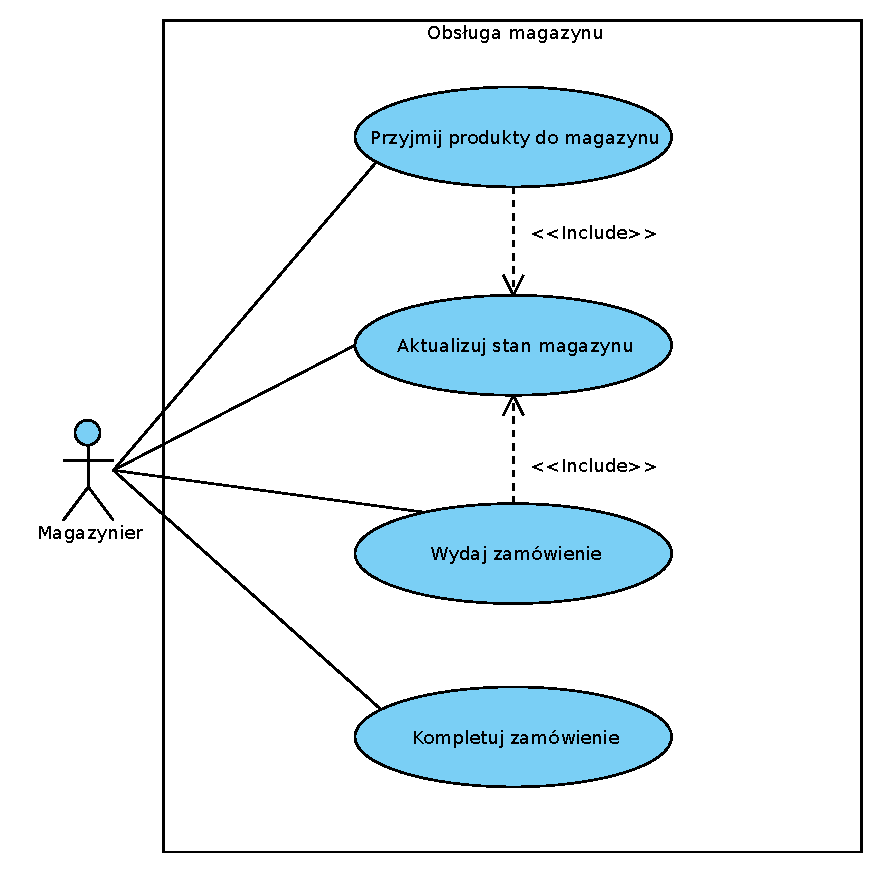
\includegraphics[width=.8\textwidth]{img/UC/magazyn.eps}
\end{figure}

\textbf{Numer i Nazwa przypadku użycia:} UC01 - Przyjmij produkty do magazynu \\
\textbf{Autor:} Magazynier\\
\textbf{Cel przypadku użycia:} Dodanie produktów recyklingu do magazynu i aktualizacja stanu magazynu \\
\textbf{Kontekst użycia:} przechowanie produktów recyklingu w magazynie\\
\textbf{Zakres:} system magazynowy \\
\textbf{Poziom:} biznesowy \\
\textbf{Aktor główny:} Magazynier \\
\textbf{Uczestnicy:} Kierowca \\
\textbf{Wyzwalacz:} dostarczenie przez kierowce produktów do magazynu \\
\textbf{Warunek początkowy:} kierowca ma produkty recyklingu, które należy zmagazynować oraz ich listę \\
\textbf{Minimalna gwarancja:} w przypadku, gdy produkty nie zostaną zmagazynowane, stan magazynu nie będzie zmieniany \\
\textbf{Główny scenariusz powodzenia:} \\
	\begin{enumerate}
		\item Kierowca przywozi produkty
		\item Magazynier układa je w magazynie
		\item Magazynier aktualizuje stan magazynu
	\end{enumerate}
\begin{figure}[H]
	\centering
	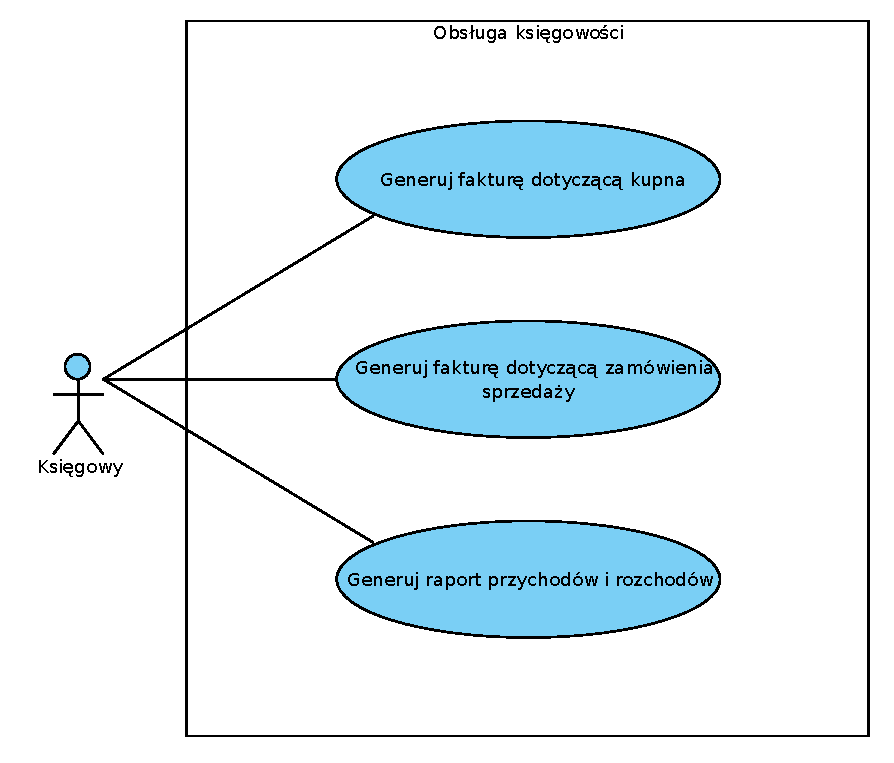
\includegraphics[width=.8\textwidth]{img/UC/ksiegowosc.eps}
\end{figure}

\textbf{Numer i Nazwa przypadku użycia:} UC02 - Wydaj zamówienie \\
\textbf{Autor:} Magazynier\\
\textbf{Cel przypadku użycia:} Wydanie kierowcy produktów, ujętych w zamówieniu \\
\textbf{Kontekst użycia:} potrzeba przetransporotowania produktów do kupca\\
\textbf{Zakres:} system magazynowy \\
\textbf{Poziom:} biznesowy \\
\textbf{Aktor główny:} Magazynier \\
\textbf{Uczestnicy:} Kierowca \\
\textbf{Wyzwalacz:} przyjazd kierowcy do magazynu \\
\textbf{Warunek początkowy:} kierowca ma zamówienie \\
\textbf{Minimalna gwarancja:} w przypadku, gdy nie można skompletować zamówienia stan magazynu się nie zmieni \\
\textbf{Główny scenariusz powodzenia:} \\
	\begin{enumerate}
		\item Kierowca przekazuje numer zamówienia magazynierowi
		\item Magazynier wydaje produkty kierowcy
		\item Magazynier uaktualnia stan magazynu
	\end{enumerate}
\textbf{Rozszerzenia:} \\
1.1 W przypadku gdy magazynier nie otrzymał wcześniej informacji o zamówieniu, kompletuje je teraz, w razie niepowodzenia produkty nie zostają wydane\\

\textbf{Numer i Nazwa przypadku użycia:} UC03 - Aktualizuj stan magazynu \\
\textbf{Autor:} Magazynier\\
\textbf{Cel przypadku użycia:} Aktualizacja danych o stanie magayznu \\
\textbf{Kontekst użycia:} utrzymywanie aktualnej informacji o ilości produktów w magazynie \\
\textbf{Zakres:} system magazynowy \\
\textbf{Poziom:} użytkowy \\
\textbf{Aktor główny:} Magazynier \\
\textbf{Wyzwalacz:} wydanie lub przyjęcie produktów \\
\textbf{Warunek początkowy:} zmiana stanu magazynu \\
\textbf{Minimalna gwarancja:} w przypadku, gdy nie można zaktualizować stanu magazynu, jego stan pozostanie niezmieniony \\
\textbf{Główny scenariusz powodzenia:} \\
	\begin{enumerate}
		\item Magazynier wpisuje informację o wydanych/przyjętych produktach
	\end{enumerate}

\textbf{Numer i Nazwa przypadku użycia:} UC04 - Kompletuj zamówienie \\
\textbf{Autor:} Magazynier\\
\textbf{Cel przypadku użycia:} Skompletowanie zamówienie w celu wydania go kierowcy \\
\textbf{Kontekst użycia:} chęć uporządkowania produktów do zamówienia w celu szybkiego ich przekazania kierowcy \\
\textbf{Zakres:} system magazynowy \\
\textbf{Poziom:} biznesowy \\
\textbf{Aktor główny:} Magazynier \\
\textbf{Wyzwalacz:} dostanie informacji o zamówieniu \\
\textbf{Warunek początkowy:} odpowiednia ilość towarów w magazynie \\
\textbf{Minimalna gwarancja:} w przypadku, gdy nie ma odpowiedniej ilości towarów w magazynie, zostanie wysłana informacja zwrotna  \\
\textbf{Główny scenariusz powodzenia:} \\
	\begin{enumerate}
		\item Magazynier otrzymuje listę towarów, które wchodzą w skład zamówienia
		\item Magazynier sprawdza czy posiada ich odpowiednią ilość
		\item Magazynier przygotowuje zamówienie
	\end{enumerate}
\textbf{Rozszerzenia:} \\
2.1. Nie można skompletować zamówienia, zostaje wysłana informacja zwrotna o nieposiadanych towarach\\

\begin{figure}[H]
	\centering
	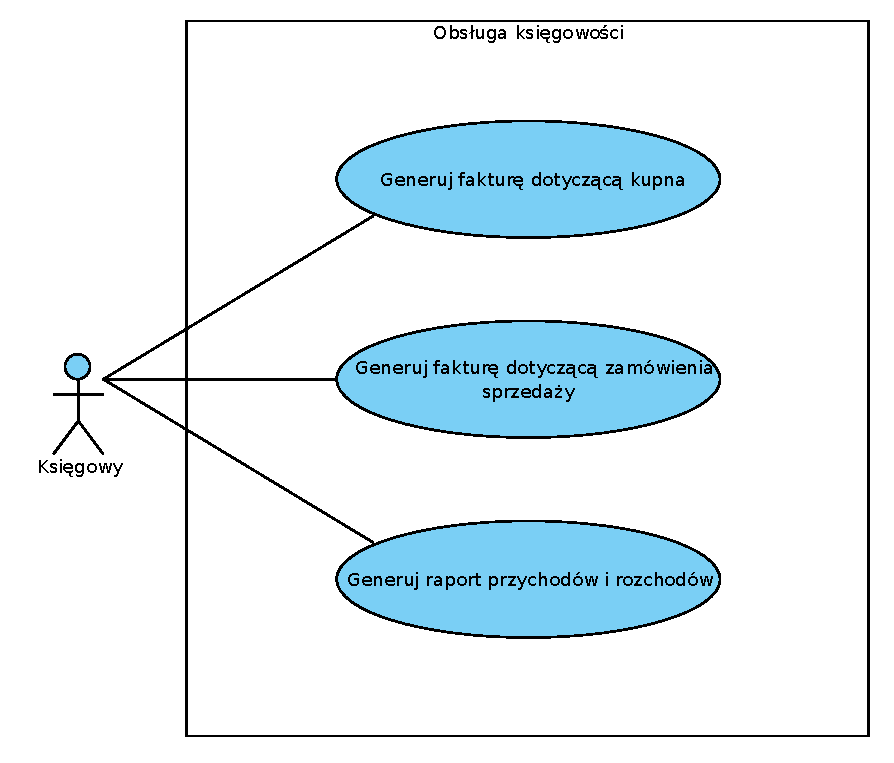
\includegraphics[width=.8\textwidth]{img/UC/ksiegowosc.eps}
\end{figure}
\begin{figure}[H]
	\centering
	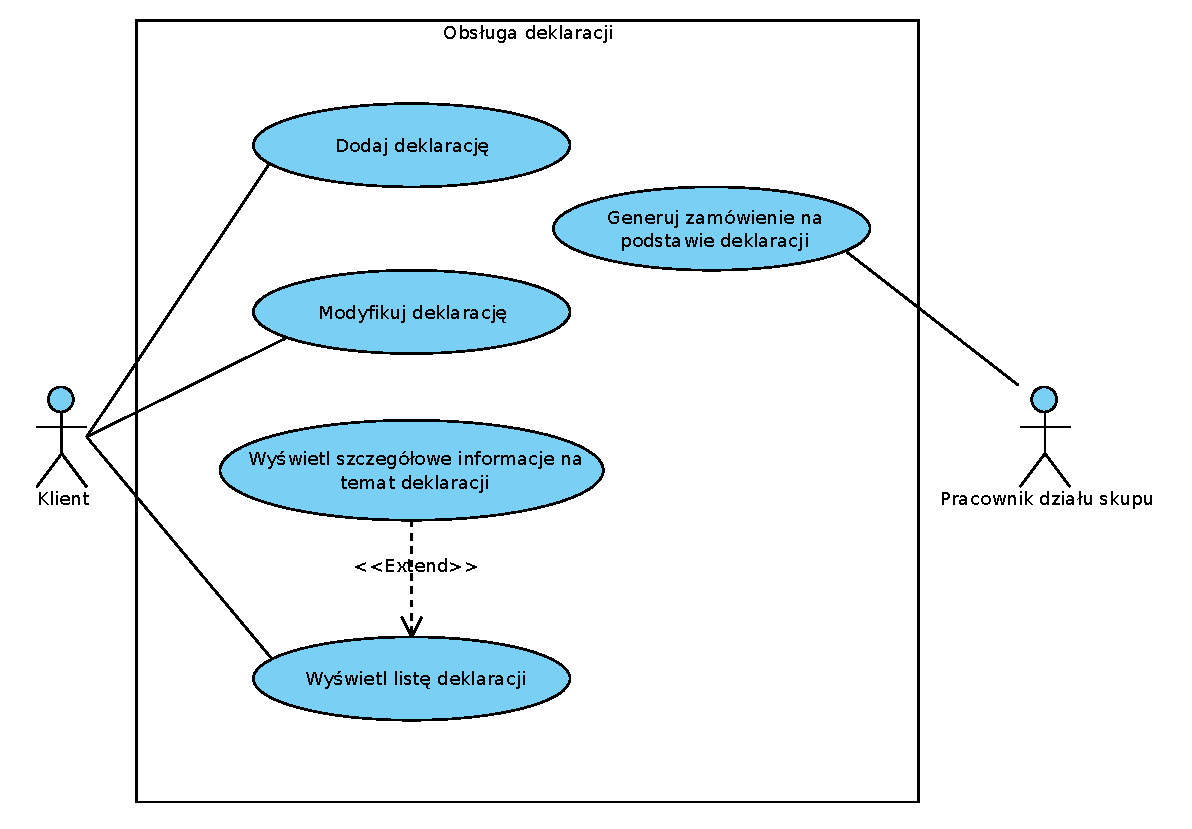
\includegraphics[width=1.1\textwidth]{img/UC/deklaracje.eps}
\end{figure}

	\subsection{Wymagania funkcjonalne dla dodatkowych funkcji systemu}
		% funkcje administracyjne, wspólne i wewnętrzne
		
\begin{enumerate}
\item Funkcje administracyjne
	\begin{itemize}
		\item użytkownik systemu z uprawnieniami administratora (administrator) może dodawać i usuwać pracowników za pomocą panelu administracyjnego (nadawać użytkownikom określone uprawnienia, niezbędne do wykonywania ich pracy z systemem)
		\item administrator ma dostęp do wszystkich deklaracji
		\item po nadaniu deklaracji statusu „przyjętej” zmian w niej może dokonywać tylko administrator na wniosek klienta
	\end{itemize}

\item Funkcje wspólne
	\begin{itemize}
		\item użytkownik może edytować deklarację do momentu nadania jej statusu „przyjętej”
		\item zależnie od uprawnień użytkownik systemu może pobrać swoje wszystkie zarchiwizowane deklaracje w wygodnym dla niego pliku
		\item użytkownik może sprawdzić stan danej przesyłki odpadów
	\end{itemize}

\item Funkcje wewnętrzne
	\begin{itemize}
		\item generowanie faktur
		\item generowanie potwierdzeń odbioru dla kierowców
		\item tworzenie kopii zapasowych
		\item pobieranie danych archiwalnych
	\end{itemize}

\end{enumerate}

	\subsection{Wymagania niefunkcjonalne}
		% z podziałem na grupy wymagań
		
\begin{enumerate}
\item Użyteczność
	\begin{itemize}
		\item interakcja z użytkownikiem powinna być czytelna
		\item użycie prostych, estetycznych i czytelnych czcionek
		\item użycie intuicyjnych kolorów, np. dla błędnych danych koloru czerwonego
		\item w miarę możliwości składanie deklaracji powinno być analogiczne do wypełniania innych formularzy internetowych
		\item bez zbyt złożonych efektów wizualnych, które będą widocznie spowalniały działanie systemu na słabszym sprzęcie
	\end{itemize}

\item Niezawodność
	\begin{itemize}
		\item czas awarii nie może być dłuższy niż dwie godziny
		\item każdy użytkownik ma dostęp do systemu z określonymi, niezbędnymi uprawnieniami
	\end{itemize}

\item Wydajność
	\begin{itemize}
		\item system będzie w stanie dodać nową deklarację w mniej niż 5s
		\item system będzie w stanie wygenerować nową fakturę w mniej niż 5s
		\item system wyeksportuje dane archiwalne o wielkości do 100 mb w mniej niż 10s
	\end{itemize}

\item Wspieralność
	\begin{itemize}
		\item system powinien być skalowalny, tj. dodanie nowej funkcji przetwarzania/przedstawienia danych podanych przez klienta nie powinno powodować zmiany wcześniej napisanego kodu
		\item system napisany będzie w języku Java
		\item strona internetowa będzie używała języka JavaScript


\item Harmonogram
	\begin{itemize}
		\item I miesiąc - analiza wymagań
		\item II, III miesiąc - projekt wstępny
		\item IV - VII miesiąc - projekt szczegółowy
		\item VIII - XII miesiąc - implementacja
	\end{itemize}


\end{enumerate}

\section{Analiza funkcjonalna systemu}

	\subsection{Diagram kontekstowy}
		
\begin{figure}[H]
	\centering
	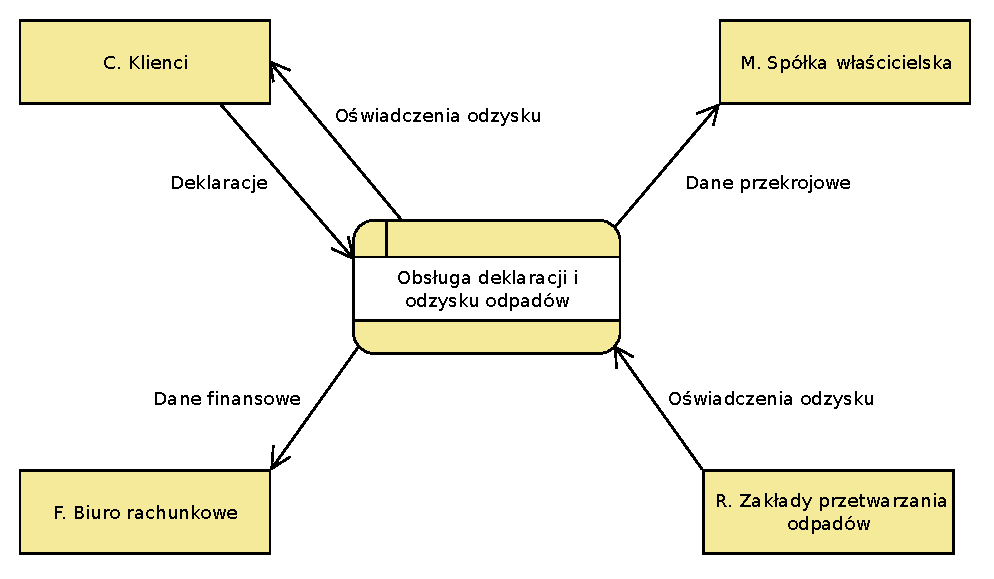
\includegraphics[width=\textwidth]{img/context.eps}
\end{figure}

	\subsection{Analiza top-down}
		
\subsubsection{Poziom 1}

\clearpage
\begin{figure}[H]
	\centering
	\includepdf[pages={1}, angle=90]{img/DFD/1_level-eps-converted-to.pdf}
\end{figure}
\clearpage

	\subsection{Opis procesów}
		\input{partials/3-analiza/3-procesy.tex}

\section{Roboczy słownik danych}
	\begin{enumerate}
\item \textbf{Dane dotyczące obsługi klienta(3.1)}
	\begin{itemize}
		\item Faktury(2.2.8) - dokument sprzedaży zawierający szczegółowe dane o transakcji.
		\item Żądanie faktury - zapytanie wywołujące transfer danych w postaci faktury.
		\item Deklaracje(2.2.3) - szczegółowe dane dotyczące tego ile towarów, które mają ulec recyklingowi wprowadził na rynek klient.
		\item Oferty sprzedaży(2.2.2) - szczegółowy spis odpadów, wraz z ich wagą, które Biosystem wykupił od firmy.
		\item Zamówienia(2.2.4) - szczegółowy spis produktów recyklingu, wraz z ich wagą/ilością które firma kupiła od Biosystem.
		\item Dane klienta(2.2.1) - Szczegółowe dane dotyczące klienta(Nazwa firmy + NIP + Adres + Numer telefonu), jeżeli klient jest zarejestrowany to także w skład tych danych wchodzi jeszcze Historia transakcji.
	\end{itemize}
\item \textbf{Dane dotyczące obsługi skupu(3.2)}
	\begin{itemize}
		\item Deklaracje - jak w 4.1
		\item Oferty sprzedaży - jak w 4.1
		\item Zakłady przetwarzania(2.2.10) - szczegółowe dane o zakładach przetwarzania z którymi Biosystem utrzymuje kontakt
		\item Żądanie - zakłady przetwarzania - żądanie o w.w. dane.
		\item Zlecenie odbioru(2.2.12) - szczegółowe dane o ilości prdouktów recyklingu, które Biosystem ma odebać z firmy przetwarzającej odpady.
		\item Oświadczenie odzysku(2.2.13) - oświadczenie potwierdzające oddzyskanie surowców wtórnych, zawiera dane o nich.
	\end{itemize}
\item \textbf{Dane dotyczące obsługi księgowości(3.3)}
	\begin{itemize}
		\item Dane klientów - jak w 4.1
		\item Faktury - jak w 4.1 
		\item Dane przekrojowe - dane dotyczące działalności firmy wygenerowane na podstawie faktur.
		\item Dane finansowe - szczegółowe dane dotyczące wszystkich transakcji finanswoych firmy(obliczane na podstawie innych dokumentów), potrzebne do rozliczenia się z urzędem skarobwym.
		\item Żądanie - dane finansowe - dokument dotyczący rozliczenia się Biosystemu z Urzędem skarbowym. 
		\item Żądanie - statystyki - żądanie statystyk dotyczące wpływów i wydatków firmy.
		\item Raporty - raport o wydatkach i dochodach firmy przygotowany dla właściciela.
	\end{itemize}
\item \textbf{Dane dotyczące obsługi magazynu(3.4)}
	\begin{itemize}
		\item Zamówienie - jak w 4.1
		\item Stan magazynu (2.2.6)- szcegółowe dane dotyczące towarów znajdujących się w magazynie.
		\item Dane o towarach (2.2.11)- dane o towarach, które przetwarza dla Biosystemu Zakład przetwarzania.
		\item Zapytanie o stan magazynu - żądanie o informacje dotyczące stanu magazynu.
	\end{itemize}
\item \textbf{Dane dotyczące obsługi kierowców(3.5)}
	\begin{itemize}
		\item Oferty sprzedaży - jak w 4.1
		\item Zapytanie o dane - zapytanie o dane klienta od którego mają być odebrane odpady, lub dostarczone produkty recyklingu.
		\item Zamówienia - jak w 4.1
	\end{itemize}
\end{enumerate}

	
\section{Analiza struktur danych w przechowywanych magazynach}
	Odwzorowanie magazynów danych z diagramów DFD(3.2.1) w bazie danych:
\begin{itemize}
	\item 3.2.1.D1 Klienci - w tabelach "Klienci" i "Klienci z umową"
	\item 3.2.1.D2 Deklaracje - w tabeli "Deklaracje"
	\item 3.2.1.D3 Faktury - są czerpane z tabeli "Transakcje", nie ma sensu trzymać ich w bazie
	\item 3.2.1.D4 Oferty sprzedaży - w tabeli "Oferty sprzedaży"
	\item 3.2.1.D5 Zamówienia - w tabeli "Zamówienia"
	\item 3.2.1.D6 Magazyn - w tabeli "Produkt"
	\item 3.2.1.D7 Oświadczenia oddzysku - są czerpane z "Zleceń przetworzenia"
	\item 3.2.1.D8 Zlecenie odbioru - są czerpane z "Ofert sprzedaży", bo wtedy Biosystem S.A jest zobowiązany od odebrania odpadów od klientów
\end{itemize}

\newcolumntype{Y}{>{\centering\arraybackslash}X}

\begin{landscape}
	\subsection{Opis relacji w tabeli krzyżowej}
	\begin{table}[H] 
		\centering
		\centerline{\begin{tabularx}{1.1\hsize}{@{}|Y|Y|Y|Y|Y|Y|Y|Y|Y|Y|Y|Y|Y@{}}
\hline
                                                     & Klienci               & Klienci z umową       & Adres                  & Historia transakcji   & Pracownik              & Oferty sprzedaży      & Zamówienia            & Deklaracje            & Odpady                 & Produkty              & Zlecenie przetworzenia odpadów &Zakład przetwarzania odpadów\\ \hline
Klienci                                              &                       & X                     & X                      & X                     &                        & X                     & X                     & X                     &                        &                       &                                                     &                                                   \\ \hline
Klienci z umową                                      & X                     &                       & X                      & X                     &                        & X                     & X                     & X                     &                        &                       &                                                     &                                                   \\ \hline
Adres                                                & X                     & X                     &                        &                       &                        &                       &                       &                       &                        &                       &                                                     & X                                                 \\ \hline
Historia negocjacji                                  &                       & X                     &                        &                       &                        &                       & X                     & X                     & X                      &                       &                                                     &                                                   \\ \hline
Pracownik                                            &                       &                       &                        &                       &                        &                       & X                     & X                     & X                      &                       & X                                                   &                                                   \\ \hline
Oferty sprzedaży                                     & X                     & X                     &                        & X                     & X                      &                       &                       &                       & X                      &                       &                                                     &                                                   \\ \hline
Zamówienia                                           & X                     & X                     &                        & X                     & X                      &                       &                       &                       &                        & X                     &                                                     &                                                   \\ \hline
Deklaracje                                           & X                     & X                     &                        & X                     & X                      &                       &                       &                       & X                      &                       &                                                     &                                                   \\ \hline
Odpady                                               &                       &                       &                        &                       &                        &                       & X                     & X                     &                        &                       & X                                                   &                                                   \\ \hline
Produkty                                             &                       &                       &                        &                       &                        & X                     &                       &                       &                        &                       &	                                                     &                                                   \\ \hline
Zlecenie przetwarzania odpadów &  &	& 	&	&	X &		 &		 &		 &X & 	                   & X                                                 \\ \hline
Zakład przetwarzania odpadów   & 	 & 	& X		 & 		 & 		  & 		 & 		 & 		 & 		  & 	 &                                            \\ \hline
		\end{tabularx}}
	\end{table}
\end{landscape}

\subsection{Encje}
	\begin{enumerate}

		\item Historia transakcji
		\begin{enumerate}
			\item ID Historia transakcji
			\item ID Klienta
			\item Zakończone transakcje
		\end{enumerate}

		\item Zakończone transakcje
		\begin{enumerate}
			\item ID zakończonej
			\item ID Transakcji
		\end{enumerate}

		\item Klienci z umową
		\begin{enumerate}
			\item ID Klienta z umową
			\item ID Klienta
			\item NIP
		\end{enumerate}

		\item Klienci
		\begin{enumerate}
			\item ID Klienta
			\item Nazwa firmy
			\item AdresID
			\item Numer telefonu
		\end{enumerate}

		\item Adres
		\begin{enumerate}
			\item ID Adres
			\item Miasto
			\item Ulica
			\item Nr budynku
			\item Kod pocztowy
		\end{enumerate}

		\item Transakcje
		\begin{enumerate}
			\item ID
			\item ID Klienta
			\item ID Transakcji
			\item ID Pracownika
		\end{enumerate}

		\item Pracownik
		\begin{enumerate}
			\item ID Pracownika
			\item Imię
			\item Nazwisko
			\item PESEL
			\item Data urodzenia
			\item Data zatrudnienia
			\item Stanowisko
			\item Bezpośredni zwierzchnik
		\end{enumerate}

		\item Oferty sprzedaży
		\begin{enumerate}
			\item ID Oferty
			\item Lista produktów recyklingu
			\item Data zamówienia
			\item Data odbioru
			\item Wartość
		\end{enumerate}

		\item Zamówienia
		\begin{enumerate}
			\item ID Zamówienia
			\item Lista odpadów
			\item Data
			\item Status
			\item Wartość
		\end{enumerate}

		\item Deklaracje
		\begin{enumerate}
			\item ID Deklaracji
			\item Lista odpadów
			\item Data
		\end{enumerate}

		\item Lista produktów recyklingu
		\begin{enumerate}
			\item ID Listy
			\item ID Produktu
			\item Waga
		\end{enumerate}

		\item Produkt
		\begin{enumerate}
			\item ID Produktu
			\item Nazwa
		\end{enumerate}

		\item Lista odpadów
		\begin{enumerate}
			\item ID Listy
			\item ID Odpadu
			\item Waga
		\end{enumerate}

		\item Odpad
		\begin{enumerate}
			\item ID Odpadu
			\item Nazwa
		\end{enumerate}
	\end{enumerate}
\begin{landscape}
	\begin{figure}
		\centering
		\centerline{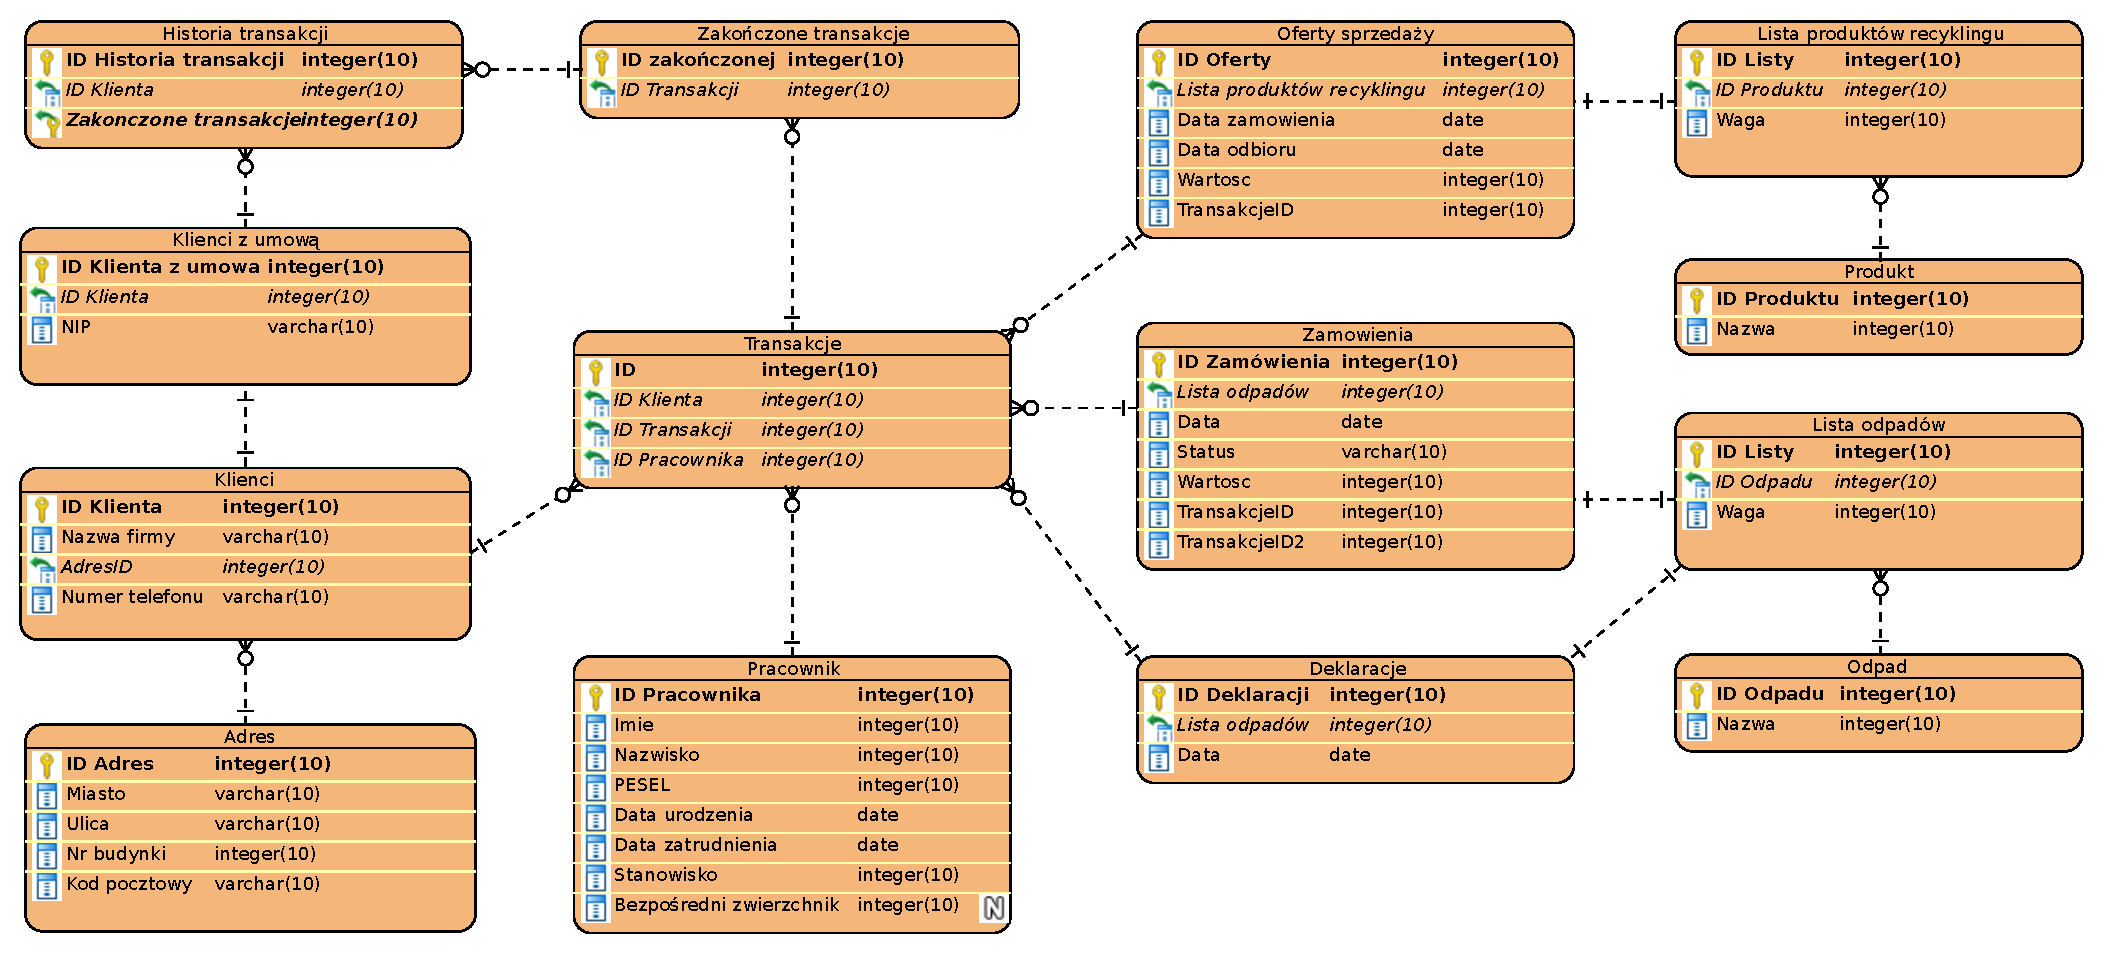
\includegraphics[width=28cm]{img/ERD.eps}}
	\end{figure}
\end{landscape}

\section{Obraz zachowania systemu w czasie}

	\begin{figure}[H]
		\centering
		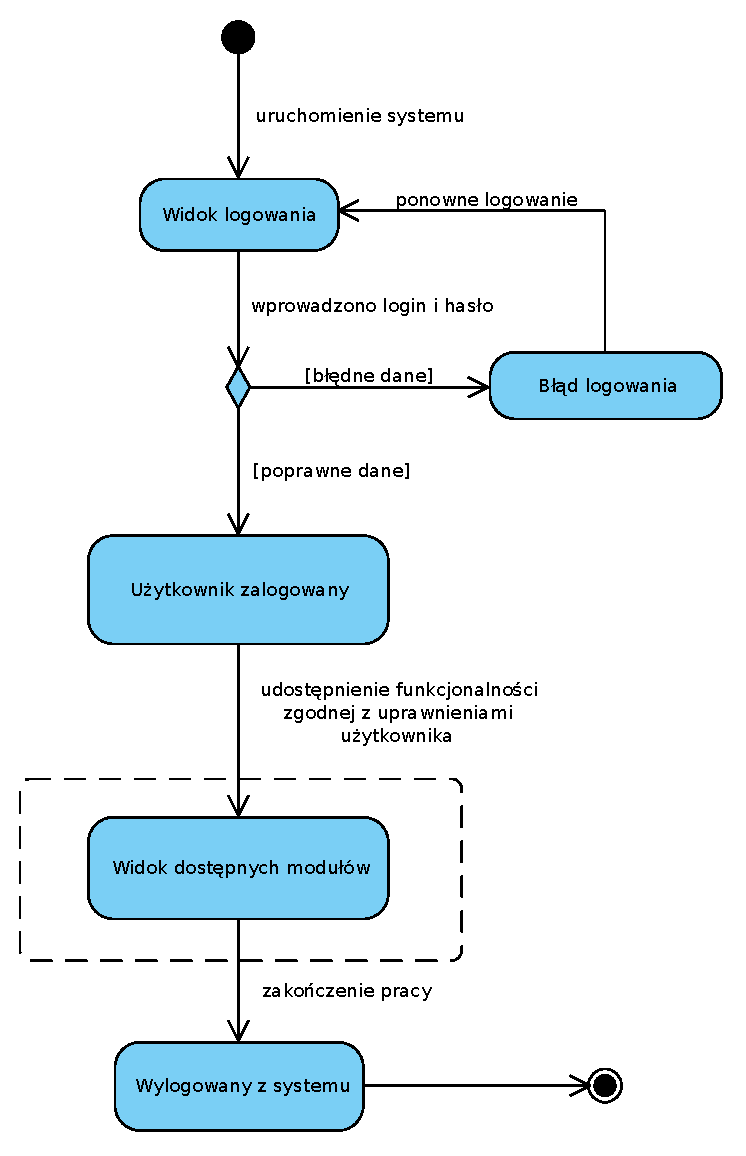
\includegraphics[width=.8\textwidth]{img/AD/STDmain.eps}
		\caption{Ogólny diagram STD}
	\end{figure}

\section{Równoważenie modeli}
	Ocena spójności wymagań użytkowników z zaprojektowanymi przez nas DFD oraz ERD nie wykazała sprzeczności, co więcej pozwoliła sądzić, że zaproponowane przez nas procesy oraz struktury danych zapewnią uzyskanie wszystkich wymaganych przez klienta funkcjonalności. Zgodność modeli ze specyfiacją jest w głównej mierze zasługą klienta, który bardzo dokładnie sprecyzował swoje wymagania. \\
Warto zauważyć, że w diagramach USE CASE skupiamy się na ogólnej funkcjonalności biznesowej systemu, upływ czasu oraz więcej szczegółów znajduje się w diagramach aktywności.



\section{Architektura systemu}
		\begin{figure}[H]
		\centering
		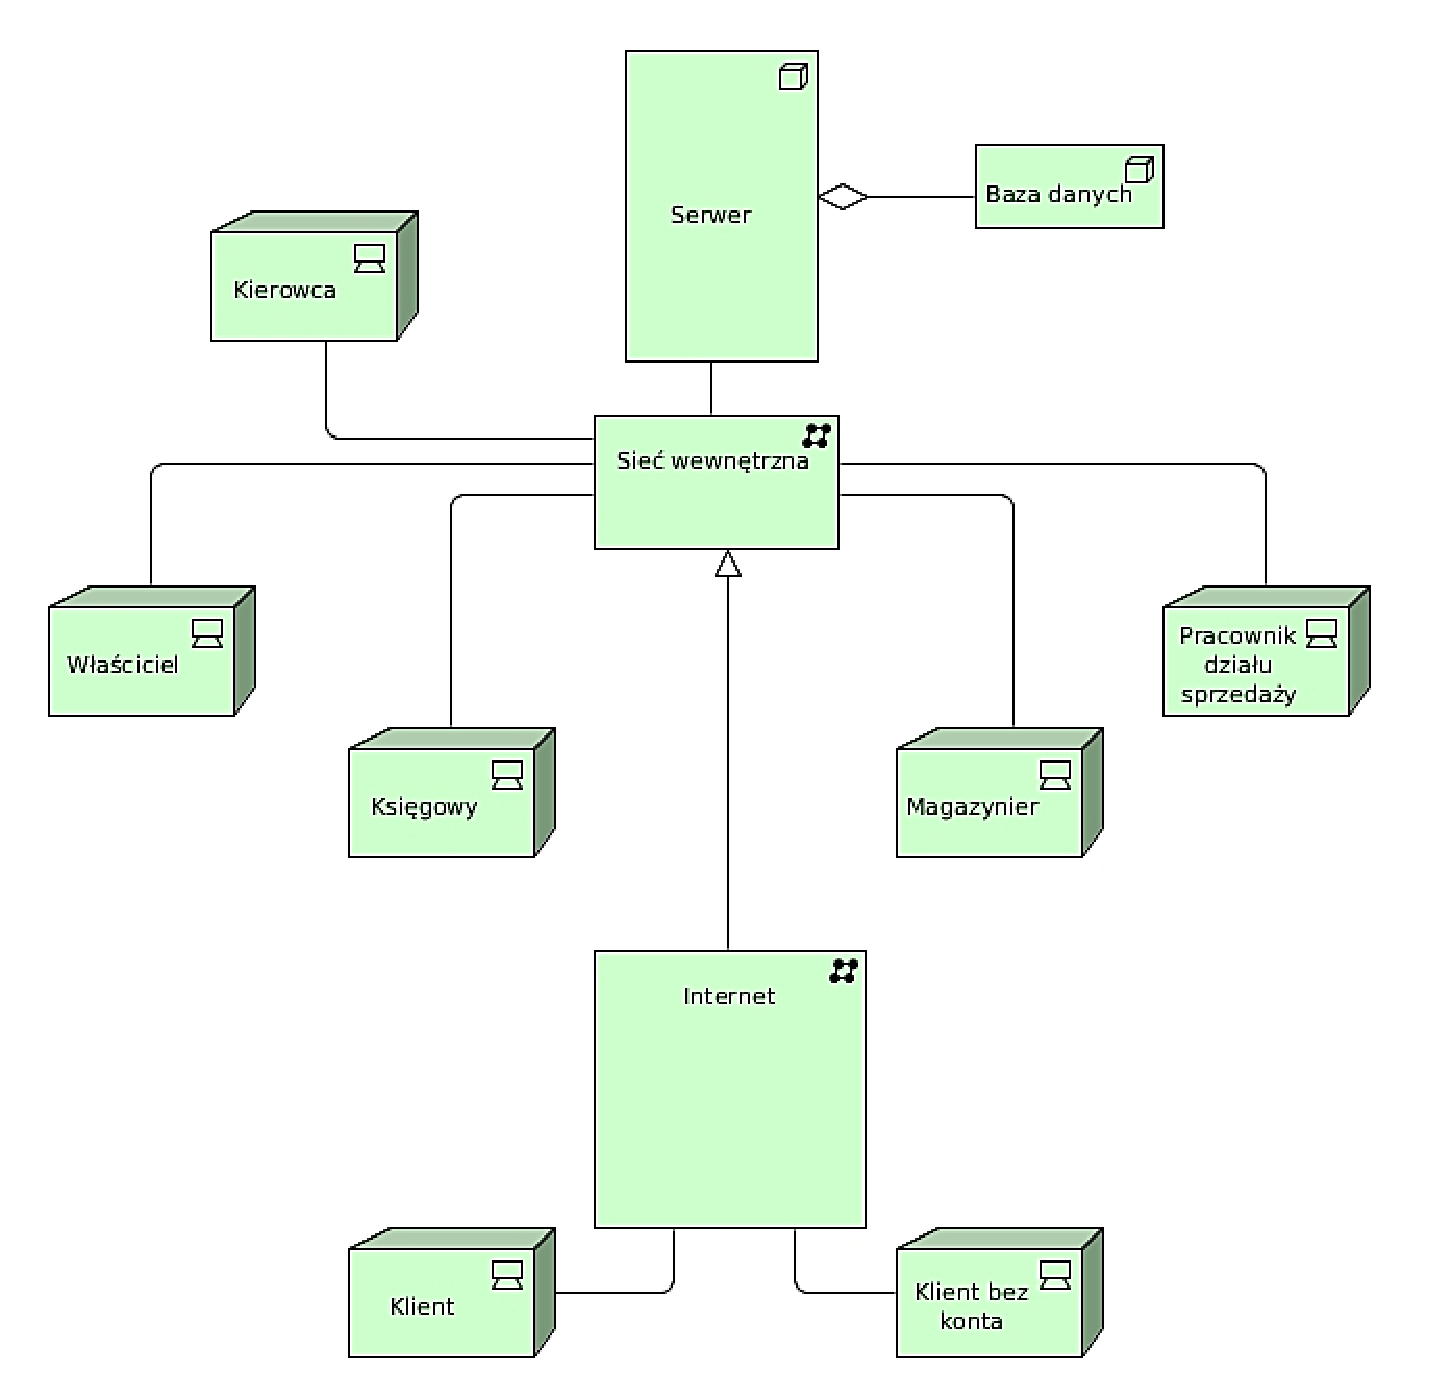
\includegraphics[width=1.1\textwidth]{img/architektura.eps}
	\end{figure}

Architektura systemu jest oparta na schemacie klient - serwer. Pracownicy firmy będą komunikowali się ze sobą w sieci wewnętrznej, natomiast klienci będą łączyli się z naszą firmą poprzez internet. System będzie działał w architekturze aplikacji webowej, obsługiwanej z poziomu przeglądarki. Dzięki temu unikniemy konieczności wymuszania instalacji dodatkowego oprogramowania przez naszych klientów, która w niewielu przypadkach mogłaby być kłopotliwa. 
	% \subsection{Architektura całego systemu}
	% \subsection{Architektura podsystemów}
	% \subsection{Wewnętrzna architektura podsystemów}

\section{Projekt interfejsu użytkownika}

	\begin{figure}[H]
		\centering
		\centerline{\includegraphics[width=\textwidth]{partials/2-wymagania/dokumenty/dane-klienta.png}}
		\caption{Formularz - dane klienta}
	\end{figure}

	\begin{figure}[H]
		\centering
		\centerline{\includegraphics[width=1.2\textwidth]{partials/2-wymagania/dokumenty/deklaracja-form.png}}
	\end{figure}

	\begin{figure}[H]
		\centering
		\centerline{\includegraphics[width=1.2\textwidth]{partials/2-wymagania/dokumenty/oferta.png}}
		\caption{Formularz - oferta sprzedaży}
	\end{figure}


% \section{Podsumowanie}

% 	\subsection{Założenia implementacyjne}

% 	\subsection{Weryfikacja projektu systemu}

% 	\subsection{Uwagi i wnioski końcowe}

%%% End document

\section{Słownik pojęć biznesowych}
	\subsection{Użytkownicy systemu}

	\paragraph{Klient z umową}\ \\
	Firma, dla której BIOSYSTEM świadczy usługi przejęcia obowiązku odzysku odpadów na podstawie umowy. Klient posiada konto w systemie umożliwiające składanie deklaracji recyklingowych. Na podstawie deklaracji pracownicy działu skupu wykupują \emph{Oświadczenia odzysku} od zewnętrznych zakładów odzysku odpadów.

	\paragraph{Klient} \ \\
	Firma lub osoba prywatna, który może zamówić odbiór odpadów za pomocą projektowanego systemu, a także kupić surowce wyprodukowane w Zakładzie Przetwarzania Zużytego Sprzętu Elektrycznego i Elektronicznego.


\subsection{Dokumenty}
	\paragraph{Deklaracja} \ \\
	Dokument składany przez \emph{Klienta z umową} dotyczący wprowadzonych do obiegu opakowań, baterii, sprzętu elektrycznego i elektronicznego oraz ich ilości i/lub wagi.

	Na podstawie deklaracji wykupowane jest \emph{Oświadczenie odzysku}.

	\paragraph{Oświadczenie odzysku} \ \\
	Dokument kupowany od \emph{Zewnętrznych Zakładów Przetwarzających Odpady}, który opisuje rodzaje odzyskanych odpadów oraz ich ilości.

	Po przejęciu obowiązku odzysku odpadów od klienta firma BIOSYSTEM zleca \emph{Zewnętrznym Zakładom Przetwarzającym Opady} odzyskanie ilości odpadów odpowiadającym wprowadzonym do obiegu przez klienta.

\subsection{Inne}
	\paragraph{Zewnętrzny Zakład Przetwarzający Odpady} \ \\
	Firma współpracująca, niezwiązana z firmą BIOSYSTEM przeprowadzająca odzysk odpadów.


\section{Załączniki}
	\subsection{Dokumenty wprowadzane i wyprowadzane z systemu}
		\includepdf[pages={1}]{partials/2-wymagania/dokumenty/deklaracja2.pdf}	
		\includepdf[pages={1}]{partials/2-wymagania/dokumenty/faktura.pdf}		
		\includepdf[pages={1}]{partials/2-wymagania/dokumenty/zlecenie.pdf}
\end{document}